
\section{Solutions for ``Application: Introduction to Cryptography''}
\noindent\textbf{\textit{ (Chapter \ref{crypt}})}\bigskip
\\
\noindent\textbf{Exercise \ref{exercise:Cryptography:encode1}:}
\begin{enumerate}[(a)]
\item
%Encode IXLOVEXMATH using the cryptosystem in Example~\ref{example:Cryptography:ex1}.
\item
%Encode the same message using the encoding function $f(n) =n \oplus 10$.
\end{enumerate}

\noindent\textbf{Exercise \ref{exercise:Cryptography:decode1}:}
\begin{enumerate}[(a)]
\item
%Decode ZLOOA WKLVA EHARQ WKHA ILQDO, which was encoded using the cryptosystem in Example~\ref{example:Cryptography:ex1}.
\item
%Decode: OFOBIDRSXQIYENYPVYGCPBYWDROROKBD, which was encoded using a shift code with a shift of 10.
\end{enumerate}

%\noindent\textbf{Exercise \ref{exercise:Cryptography:}:} %KW not named
%\begin{enumerate}[(a)]
%\item
%The following is a ciphertext that was encoded using a shift code with a shift of 18.

%FWHKYVOGVFGCVQWFIHOKYVQGVFGCVHSPOKYVQGVFGCV

\noindent\textbf{Exercise \ref{exercise:Cryptography:plaintext1}:}  
%%The following ciphertext was encoded using a shift code. Both the letters E and I are encoded as vowels. 
%
%%IWPDAIWPEYOEOPDAMQAAJKBPDAOYEAJYAOYWNHBCWQOO
%
%\noindent
%Find the plaintext.

\noindent\textbf{Exercise \ref{exercise:Cryptography:plaintext2}:}
%In the following shift-coded ciphertext,  one of the double-letter patterns represents `ss'. 
%
%SGD DRRDMBD NE LZSGDLZSHBR HR HM HSR EQDDCNL. FDNQF BZMSNQ
%
%\noindent
%Find the plaintext.

%\noindent\textbf{Exercise \ref{exercise:Cryptography:}:} %KW not named
%\begin{enumerate}[(a)]
%\item
%For the English alphabet, how many different shift codes are there?
%\item
%Thai script has 44 letters. How many different shift codes are there for the Thai language?
%\end{enumerate}

%\noindent\textbf{Exercise \ref{exercise:Cryptography:}:} %KW not named
%\begin{enumerate}[(a)]
%\item
%Which of the numbers 0, 1, 2, $\dots$, 10 have inverses mod 26?
%\item
%For the numbers in (a) which have inverses mod 26, compute the inverses.
%\end{enumerate}

\noindent\textbf{Exercise \ref{exercise:Cryptography:affine1}:}
%Find the decoding function for the following  affine encoding functions (used on the English alphabet).
\begin{enumerate}[(a)]
\item
%$f(n)=(3 \odot n) \oplus 14$
\item
%$f(n)=(5 \odot n) \oplus 15$
\item
%$f(n)=(7 \odot n) \oplus 23$
\end{enumerate}

%\noindent\textbf{Exercise \ref{exercise:Cryptography:}:} %KW not named
% Show that the  general formula for the decoding function for $f(n) = (a \odot n) \oplus b$ is
%$$
%f^{-1}(m) = (a^{-1} \odot m)  \ominus (a^{-1}\odot b).
%$$
% (That is, show that $f \compose f^{-1}(m)=m$, and $ f^{-1}\compose  f(n) =  n$. Note that  $n$ and $m$ are \emph{variables}, while $a$ and $b$ are \emph{constants} which characterize the encoding function.)

\noindent\textbf{Exercise \ref{exercise:Cryptography:affine2}:}
%For each of the following functions, (i) determine whether the function is a valid encoding function; (ii) if the function is valid, find the decoding function. (Assume the function is working on an alphabet with 26 letters.)
\begin{enumerate}[(a)]
\item
%$f(n) = (4 \odot n) \oplus 7$
\item
%$f(n) = (5 \odot n) \oplus 13$
\item
%$f(n) = (11 \odot n) \oplus 14$
\item
%$f(n) = (13 \odot n) \oplus 22$
\end{enumerate}

\noindent\textbf{Exercise \ref{exercise:Cryptography:english}:}
\begin{enumerate}[(a)]
\item
%The general form for an affine cryptosystem encoding function is $f(n) = (a \odot n) \oplus  b$. How many different possible values of $a$ are there, for an affine cryptosystem that works on the English alphabet of 26 letters?
\item
%For the same situation as (a), how many different possible values are there for $b$?
\item
%What is the total number of affine cryptosystems that work on an alphabet of 26 letters?
\end{enumerate}

%\noindent\textbf{Exercise \ref{exercise:Cryptography:}:} %KW not named
%The Spanish alphabet has 29 letters. Give answers to parts (a), (b), and (c) of Exercise~\ref{exercise:Cryptography:english}, but with the Spanish alphabet instead of the English alphabet.

%\noindent\textbf{Exercise \ref{exercise:Cryptography:}:} %KW not named
%The Hebrew alphabet has  22 letters. Give answers to parts (a), (b), and (c) of Exercise~\ref{exercise:Cryptography:english}, but with the Hebrew alphabet instead of the English alphabet.

%\noindent\textbf{Exercise \ref{exercise:Cryptography:}:} %KW not named
%Suppose that the encoding function for an affine cryptosystem is $f(n) = (a \odot n) \oplus  b$, and the decoding function is 
%$f^{-1}(m) = (a' \odot m) \oplus  b'$. Suppose that a different cryptosystem uses the encoding function $g(n) = (a' \odot n) \oplus  b'$. What is the decoding function for this second cryptosystem?

%\noindent\textbf{Exercise \ref{exercise:Cryptography:}:} %KW not named
%\begin{enumerate}[(a)]
%\item
%The following message was encoded using an affine cryptosystem that encodes A as M and B as B. 
%\medskip
%
%CKMYCZMLCOZCWKOHUCKDOHLMZLLNMZGZOEVUFYU\\
%
%\noindent
%Find the plaintext.
%\item
%The following message was encoded using an affine cryptosystem that encodes A as G and C as C.
%\medskip
%
%MQTNOELNWNETEHCEWHISCFKYHHFYKGCCEIPXQWFISCF
%
%\noindent
%Find the plaintext.
%\item
%The following message was encoded using an affine cryptosystem that encodes R as S and S as D.
%\medskip
%
%OMFMFNSOMNDSFNDLADOMNOSFNDLAJNAALOZAUFSDONAU
%
%\noindent
%Find the plaintext.
%
%\item
%The following message was encoded using an affine cryptosystem that encodes M as N and O as D.
%\medskip
%
%NVEMBNVEHLJHJEMBNZJHLDWOBVJDI
%
%\noindent
%Find the plaintext.
%
%\end{enumerate}

%\noindent\textbf{Exercise \ref{exercise:Cryptography:}:} %KW not named
%What is the total number of monoalphabetic cryptosystems?

\noindent\textbf{Exercise \ref{exercise:Cryptography:mod_mult}:}
%Perform the following operations using modular matrix multiplication (mod 26):
\begin{multicols}{2}
\begin{enumerate}[(a)]
\item
%$\left(
%\begin{array}{cc}
%5 & 6 \\
%7 & 8
%\end{array}
%\right)
%\left(
%\begin{array}{c}
%4 \\
%4
%\end{array}
%\right)$

\item
%$\left(
%\begin{array}{cc}
%1 & 13 \\
%16 & 2
%\end{array}
%\right)
%\left(
%\begin{array}{c}
%3 \\
%1
%\end{array}
%\right)$

\item
%$\left(
%\begin{array}{cc}
%12 & 4 \\
%13 & 5
%\end{array}
%\right)
%\left(
%\begin{array}{cc}
%2 &1 \\
%20 & 20 
%\end{array}
%\right)$

\item
%$\left(
%\begin{array}{cc}
%13 & 2 \\
%2 & 13
%\end{array}
%\right)
%\left(
%\begin{array}{cc}
%2 &13 \\
%13 & 2 
%\end{array}
%\right)$
\end{enumerate}
\end{multicols}

%\noindent\textbf{Exercise \ref{exercise:Cryptography:}:} %KW not named
%Suppose that $(a \odot d) \, \ominus \, (b \odot c)$ has an inverse in ${\Bbb Z}_{26}$: that is to say, suppose there is a $k \in  {\Bbb Z}_{26}$ such that $k \odot ((a \odot d) \, \ominus \, (b \odot c)) = 1$.  Show that the matrices:
%$$
%A = \left( \begin{array}{cc} a & b \\ c & d \end{array} \right)~~~\text{and}~~~
%B=
%\left( \begin{array}{cc}  k \odot d & - k \odot b \\ - k \odot c &  k \odot a \end{array} \right)$$
%are inverses of each other  in ${\Bbb Z}_{26}$.  That is, show that $AB = BA = I$ under matrix multiplication mod 26.

\noindent\textbf{Exercise \ref{exercise:Cryptography:mat1}:}
%Suppose that $A = \left( \begin{array}{cc} a & b \\ c & d \end{array} \right)$ is a matrix with entries in ${\Bbb Z}_{26}$, such that  $(a \odot d)  \ominus (b \odot c)$ has no inverse in ${\Bbb Z}_{26}$. Show that $A$ has no inverse in  ${\Bbb Z}_{26}$.
%\hyperref[sec:Cryptography:Hints]{(*Hint*)}

\noindent\textbf{Exercise \ref{exercise:Cryptography:minv}:}
%Find matrix inverses in ${\Bbb Z}_{26}$ for the following matrices. If no inverse exists, then prove there is no inverse.
\begin{multicols}{2}
\begin{enumerate}[(a)]
\item
%$\left( \begin{array}{cc} 9 & 2 \\ 20 & 31 \end{array} \right)$
\item
%$\left( \begin{array}{cc} 2 & 3 \\ 23 & 2 \end{array} \right)$
\item
%$\left( \begin{array}{cc} 4 & 11 \\ 3 & 2 \end{array} \right)$
\item
%$\left( \begin{array}{cc} 2 & 2 \\ 3 & 4 \end{array} \right)$
\end{enumerate}
\end{multicols}

 %\noindent\textbf{Exercise \ref{exercise:Cryptography:}:} %KW not named
%For the same matrices as in Exercise~\ref{exercise:Cryptography:minv}, find the matrix inverses in ${\Bbb Z}_{29}$.

%\noindent\textbf{Exercise \ref{exercise:Cryptography:}:} %KW not named
%Given that
%$$
%A =
%\left(
%\begin{array}{cc}
%3 & 4 \\
%2 & 3
%\end{array}
%\right),~~ \text{and~} {\bold b} = \left( \begin{array}{c} 2 \\ 5 \end{array}\right).$$
%\begin{enumerate}[(a)]
%\item
%Use the encryption function $f({\bold p}) = A {\bold p} + {\bold b}$
%to encode the message CRYPTOLOGY.  
%\item
%What is the decoding function?  
%\end{enumerate}
 
\noindent\textbf{Exercise \ref{exercise:Cryptography:EngShift}:}
%In this exercise, you will use a spreadsheet to create an automated shift encoder for English. Please refer to Figure~\ref{fig:AutoShiftEnc} for guidance:
%\begin{figure}[h]
%\center{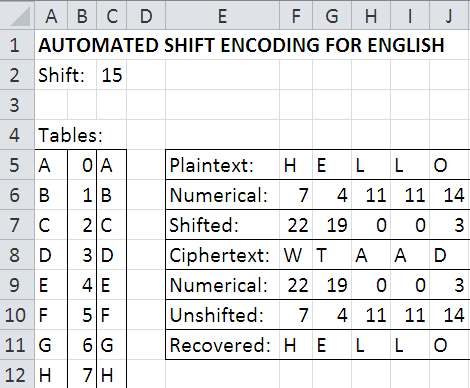
\includegraphics[width=3.0in]{images/AutoShiftEnc.png}}
%\caption{Automatic shift encoder for English.}
%\label{fig:AutoShiftEnc}
%\end{figure}
\begin{enumerate}[(i)]
\item
%Put the Shift value in cell C2.
\item
%Put the alphabet (starting with A), numerical values for the letters (starting with 0), and the alphabet again in columns A, B, C starting on line 5.
\item
%Type your plaintext in row 5, starting in column F.
\item
%Row 6 beginning in column F contains the numerical values for the plaintext. The formula in cell F6 is: ``=VLOOKUP(F5, \$A\$5:\$B\$30,2)''. The significance of this formula is as follows:
\begin{itemize}
\item
%The function VLOOKUP means that the program will look up a given value in a given table;
\item
%The F5 is the first argument of VLOOKUP, which means that the value being looked up is in cell F5;
\item
%The \$A\$5:\$B\$30 is the second argument of VLOOKUP, which means that it represents the cells containing the table that the value will be looked up in.  The dollar signs are used to guarantee that the table will remain fixed when the formula is copied and pasted into another cell;
%The 2 which is the third lookup of VLOOKUP indicates that the value in the second column in the same row as the looked-up value is placed in the cell where the formula is located.
\end{itemize}
\item
%Row 7 beginning in column F gives the encoded numerical values. The formula in cell F7 is ``=MOD(F6+\$C\$2,26)''.  The dollar signs on C2 guarantee that when the formula is copied, the shift still refers to the value in C2.
\item
%Row 8 beginning in column F gives the ciphertext.  The formula in cell F8 is: ``=VLOOKUP(F7,\$B\$5:\$C\$30,2)''. 
\item
%Rows 9,10, and 11 are similar to rows 6,7,8 respectively. Try to do this yourself. 
\end{enumerate}
%Once you have completed the formulas, select cells F6 through J11, and use the spreadsheet's ``Fill Right'' capability to carry the formulas to the other columns.  (If your plaintext is longer, you can select more columns and fill right.

%\noindent\textbf{Exercise \ref{exercise:Cryptography:}:} %KW not named
%The Spanish alphabet has 3 more letters than English:  `Ch' (comes after C in the alphabet), `Ll'  (comes after L in the alphabet), and `Nn' (comes after N).  Modify the sheet you created in Exercise \ref{exercise:Cryptography:EngShift} to make a Spanish language shift encoder.  Use your sheet to decode the following message:
%
%MS KIUPVA	UID NIKPS VA MD DPMUBChM MS UMQACh
%
%(Note that `Ch' counts as a single letter.)

%\noindent\textbf{Exercise \ref{exercise:Cryptography:}:} %KW not named
%Create a spreadsheet that can perform any affine encoding on English plaintext.  You may model your spreadsheet on the sheet in Figure~\ref{fig:affine}.  Use your spreadsheet to decode the following message:
%
%
%EMBNDOBFDZXIDPEMBSBJJJZOBFDZVOBUDSEVHOB
%
%which was encoded using an affine encoding function with $b=21$.
%\begin{figure}[h]
%\center{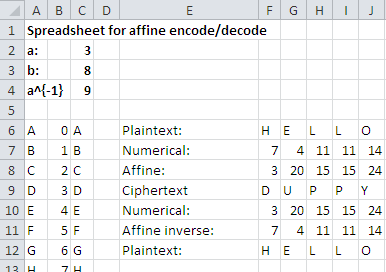
\includegraphics[width=3.5in]{images/Affine.png}}
%\caption{Automatic affine encoder for English.}
%\label{fig:affine}
%\end{figure}

%\noindent\textbf{Exercise \ref{exercise:Cryptography:}:} %KW not named
%In order to decode an affine cryptosystem on English letters with encoding function $f(p) = (a\odot p) \oplus b$, it is necessary to find the inverse of $a$ under multiplication mod 26. We have ways of finding inverses of individual numbers.  But we can also use spreadsheet software  to find all inverses in one fell swoop as described below.
%
%Open a sheet in  your favorite spreadsheet software (Excel, LibreOffice, or OpenOffice). Put the numbers 0 through 25 in column A, starting at row 3, and also in row 2 starting in column B. To fill up the table, put the formula ``=MOD(\$A3*B\$2,26)'' in cell B3, as shown in Figure~\ref{fig:mod26mult}. This formula causes the software to take the product of the contents of cells A3 and B2, and put the result mod 26 into cell B3.  The dollar signs are important: these indicate ``fixed reference''.  For example, the `\$A3' means that when this formula is copied to other cells, the reference to column A remains unchanged while the column may change. On the other hand, the `B\$2' means that when the formula is copied to other cells, the reference to column 2 remains unchanged.
%
%At this point, select the range of cells from B3 to AA28 (this will be a  square region of $26 \times 26$ cells. Use your spreadsheet's ``Fill down'' and ``Fill right'' feature to fill all the cells in this region. The location of all of the `1''s in this table shows all of the inverses.  For example, there is a '1' in the row labeled 9 and column labeled 3.  This means that 9 and 3 are inverses of each other mod 26.
%
%Use this spreadsheet table to create a 2-column table: in the first column, put the numbers 0 through 26, and in the second column, put the inverses (if the number has no inverse, just put a `$-$').
%\begin{figure}[h]
%\center{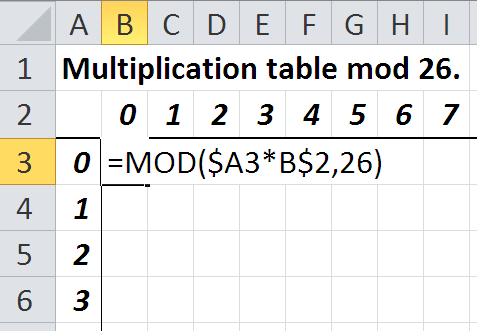
\includegraphics[width=2.25in]{images/MultMod26.png}}
%\caption{Mod 26 multiplication table.}
%\label{fig:mod26mult}
%\end{figure}

%\noindent\textbf{Exercise \ref{exercise:Cryptography:}:} %KW not named
%Following the previous exercise, find all inverses of the numbers mod 29 (this can be used in affine encoding of Spanish, which has 29 letters).

%\noindent\textbf{Exercise \ref{exercise:Cryptography:}:} %KW not named
%Make a spreadsheet that can do polyalphabetic coding.  you may base your sheet's design on Figure~\ref{fig:polycrypto}. The figure shows the encoding of the word CRYPTOLOGY using 
%$A = \left(
%\begin{array}{cc}
%3 & 5 \\
%1 & 2
%\end{array}
%\right)$, and ${\bold b} = \left( \begin{array}{c} 2 \\ 2 \end{array}\right).$ 
%
%Use your spreadsheet to decode the following words that were encoded using $f({\bold p}) = A {\bold p} + {\bold b}$ with the given $A$ and ${\bold b}$.
%\begin{enumerate}[(a)]
%\item
%VVDGOFOKLY, $A= \left(
%\begin{array}{cc}
%13 & 5 \\
%9 & 2
%\end{array}
%\right)$, and ${\bold b} = \left( \begin{array}{c} 7 \\ 13 \end{array}\right).$ 
%\item
%VWFGTWQKTA, $A= \left(
%\begin{array}{cc}
%17 & 13 \\
%6 & 3
%\end{array}
%\right)$, and ${\bold b} = \left( \begin{array}{c} 14 \\ 18 \end{array}\right).$ 
%\item
%EXUFQPRRGA, $A= \left(
%\begin{array}{cc}
%3 & 4 \\
%5 & 7
%\end{array}
%\right)$, and ${\bold b} = \left( \begin{array}{c} 4 \\ 8 \end{array}\right).$ 
%\end{enumerate}
%\begin{figure}[h]
%\center{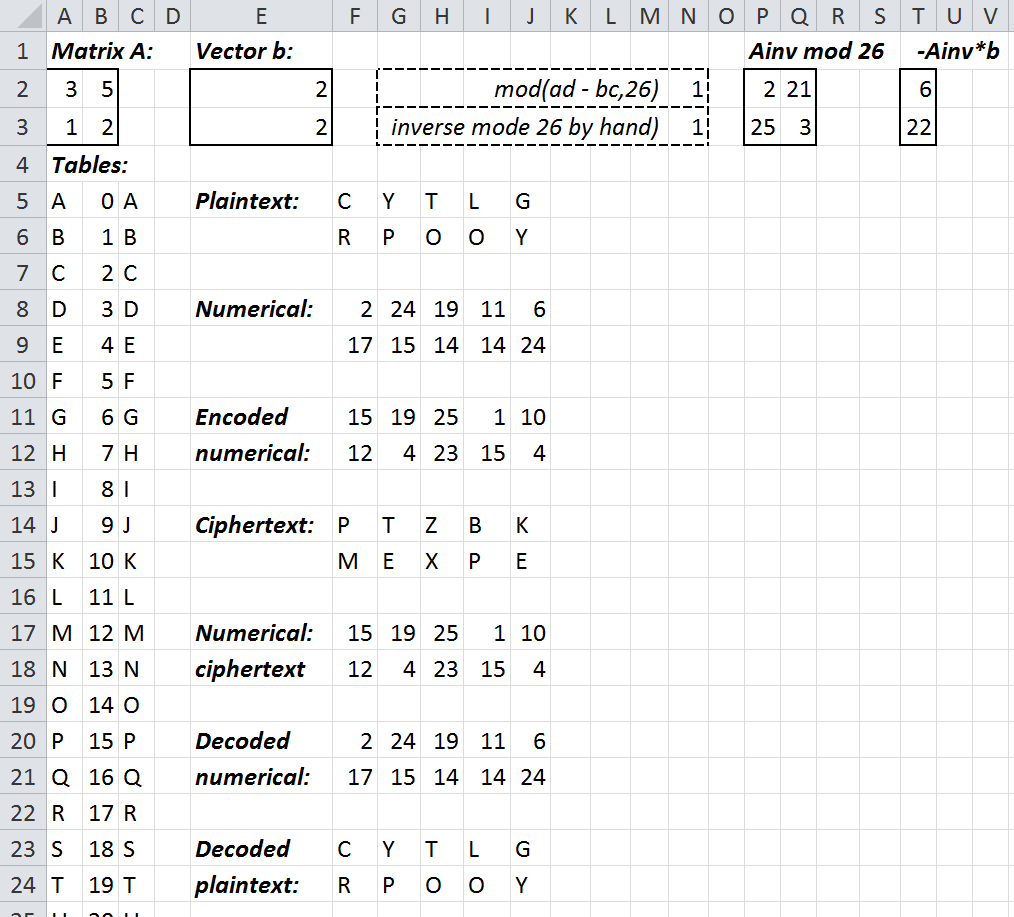
\includegraphics[width=5in]{images/polycrypto2.png}}
%\caption{(Semi-)automatic polyalphabetic encoder/decoder for English. Note that cell N3 is entered by hand, based on the value in N2.}
%\label{fig:polycrypto}
%\end{figure}
 
\noindent\textbf{Exercise \ref{exercise:Cryptography:primes}:}
%Show that if $p$ and $q$ are primes, then the number of positive integers less than $pq$ which are relatively prime to $pq$ is $(p-1)(q-1)$.
%\hyperref[sec:Cryptography:Hints]{(*Hint*)}

\noindent\textbf{Exercise \ref{exercise:Cryptography:power}:}
%This problem demonstrates a fast method for computing very large powers of numbers in modular arithmetic using a spreadsheet.  You will need this method in order to do the subsequent problems. We will demonstrate the method by computing $\bmod(23^{485} ,617)$.
\begin{enumerate}[(a)]
\item
%Use a spreadsheet to compute the following sequence of numbers:
%\[ 23, \bmod(23^2 ,617),\bmod(23^4 ,617),\ldots,\bmod(23^{256} ,617) \]
%Note that each power of 23 in this series is the  \emph{square} of the previous power.  So to compute any number in this series, square the previous number and reduce mod 617.  You may use the MOD spreadsheet function.  It is easiest to put all the numbers in a single column. (This way, you can use the spreadsheet's ``Fill down'' feature.)
\item  
%Write 485 as a sum of powers of 2.  (This is the same thing as finding the \emph{binary expansion} of 485.)
\item 
%Using the results of (b), identify a set of entries from the table you found in part (a), such that the product of these entries is equivalent to $23^{485}  \pmod{617}$.
%\hyperref[sec:Cryptography:Hints]{(*Hint*)}
\item 
%Use your result from (c) to compute $\bmod(23^{485} ,617)$.
\end{enumerate}

\noindent\textbf{Exercise \ref{exercise:Cryptography:powerplus}:}
%Building off the previous exercise, create a spreadsheet that can compute $\bmod(x^{q},n)$ for general $x,q,n$.  You may follow the pattern of the spreadsheet in Figure~\ref{fig:LargePowMod}.  Some of the formulas in the spreadsheet are:
\begin{itemize}
\item
%Cell A8: ~~=B3
\item
%Cell B8: ~~=MOD(A8,2)
\item
%Cell A9: ~~=(A8 - B8)/2
\item
%Cell D9: ~~ = D8*2
\item
%Cell E9: ~~ = MOD(E8*E8, \$B\$4)
\item
%Cell F8: ~~ = B8
\item
%Cell G8: ~~ = E8$\widehat{~~}$F8
\item
%Cell H8: ~~ = G8
\item
%Cell H9: ~~ = MOD(G9*H8,\$B\$4)
\end{itemize}
%You may obtain the rest of the formulas using the spreadsheet's ``fill down'' capability.
%
%\begin{figure}[h]
%\center{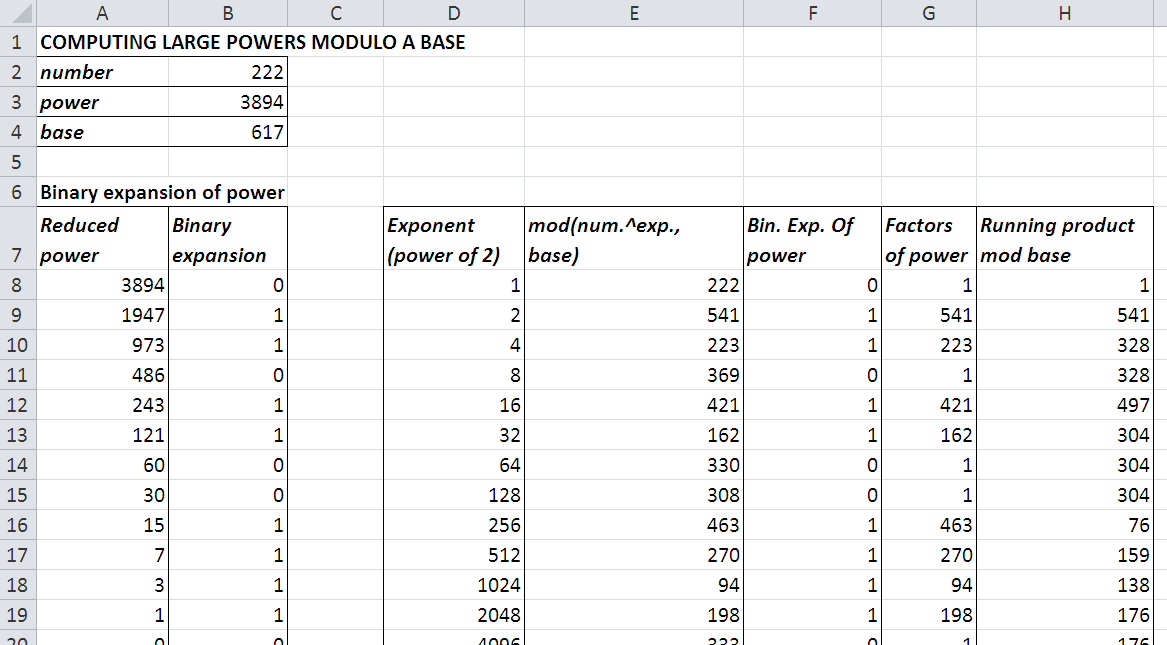
\includegraphics[width=5.5in]{images/LargePowMod.png}}
%\caption{Spreadsheet for taking large powers modulo a given base.}
%\label{fig:LargePowMod}
%\end{figure}

\noindent\textbf{Exercise \ref{exercise:Cryptography:RSA_E}:}
%Using your spreadsheet from the previous exercise, encrypt each of the following plaintexts using RSA. Before encoding, divide the plaintext
%into blocks of integers of length 2;  that is, if the plaintext is $142528$, encode 
%14, 25, and 28 separately.
% 
\begin{enumerate}[(a)]
  \item
%$n = 3551, E = 629$, plaintext = 31
 \item
%$n = 2257, E = 47, $ plaintext  = 23
 \item
%$n = 120979, E = 13251,$ plaintext = 142371
\item
%$n = 45629, E = 781,$ plaintext = 231561
\end{enumerate}

 
\noindent\textbf{Exercise \ref{exercise:Cryptography:RSA_D}:}
%Decrypt each of the following RSA messages $y$. (In this case, do not break $y$ into blocks--decode the entire number.)
% 
 \begin{enumerate}[(a)]
\item
 %$n = 3551, D = 1997, y = 2791$
 \item
%$n = 5893, D = 81, y = 34$
 \item
%$n = 120979, D = 27331, y = 112135$
 \item
%$n = 79403, D = 671, y = 129381$
 \end{enumerate}

%\noindent\textbf{Exercise \ref{exercise:Cryptography:}:} %KW not named
%Encrypted messages are often divided into blocks of $n$ letters. A
%message such as THE WORLD WONDERS WHY might be encrypted as 
%JIW OCFRJ LPOEVYQ IOC but sent as JIW OCF RJL POE VYQ
%IOC.  What are the advantages of using blocks of $n$ letters? 
 
%\noindent\textbf{Exercise \ref{exercise:Cryptography:}:} %KW not named
%Construct an RSA cryptosystem as follows:
%\begin{enumerate}[(a)]
%\item
%On the web, find two four-digit primes
%\item
%Use these primes to compute $n$ and $m$.
%\item
%Choose a value of $E$ which is less than $m$, and use you Diophantine Equation spreadsheet (Exercise~\ref{exercise:ModularArithmetic:DiophantineSS} in the Modular Arithmetic chapter) to find the inverse $D$ under multiplication mod $m$.  If it turns out that $E$ is not relatively prime to $m$, try again.
%\item
%Test your cryptosystem by encoding `123', and then decoding it. To encode, use the spreadsheet that you 
%created in Exercise~\ref{exercise:Cryptography:powerplus} earlier in this chapter. To decode, make another copy of the same sheet.
%\end{enumerate}

\noindent\textbf{Exercise \ref{exercise:Cryptography:brute}:}
%To test whether the number $n$ is a prime, you divide $n$ all the integers $1,2,3, \dots$ up to $a$, and see if any of them divides evenly.  How large does $a$ have to be in order to guarantee that $n$ really is a prime?
%\hyperref[sec:Cryptography:Hints]{(*Hint*)}

\noindent\textbf{Exercise \ref{exercise:Cryptography:EulerTotient}:}
%Using the same reasoning as above, show that after dividing by $2,3,5$ the number of additional divisions required to test for primality is approximately:
%$$a\left(1 - \frac{1}{2}\right) \left(1 - \frac{1}{3}\right)\left( 1 - \frac{1}{5} \right).$

\noindent\textbf{Exercise \ref{exercise:Cryptography:Fermat}:}
%Let $n= ab$ be an odd composite number. Prove that $n$ can be written
%as the difference of two perfect squares :
%$$
%n = x^2 - y^2 = (x-y)(x+y),
%$$
%where both $x$ and $y$ are greater than 1. Consequently, a positive odd integer can be factored exactly when we
%can find integers $x$ and $y$ such that $n = x^2 - y^2$.
%\hyperref[sec:Cryptography:Hints]{(*Hint*)} 

\noindent\textbf{Exercise \ref{exercise:Cryptography:smallest_value}:}
%In the formula  $n = x^2 - y^2 = (x-y)(x+y)$,  what is the smallest possible value for $x$ that needs to be tested?
%\hyperref[sec:Cryptography:Hints]{(*Hint*)}

\noindent\textbf{Exercise \ref{exercise:Cryptography:FermatEfficient}:}
\begin{enumerate}[(a)]
\item
%Assuming that $n$ is an odd number, show that if $x$ is odd then $y$ is even, and if $x$ is even then $y$ is odd.
%\hyperref[sec:Cryptography:Hints]{(*Hint*)}
\item
%Show that for any odd number $m$, then $\mod(m^2,4) = 1$.
%\hyperref[sec:Cryptography:Hints]{(*Hint*)}
\item
%Let $m = x + y$. Show that $m$ is odd, and that we can rewrite  $n  = (x-y)(x+y)$ as: $n = m(m-2y)$. 
\item
%Show that if $\mod(n,4)=1$, then $y$ must be even.
%\hyperref[sec:Cryptography:Hints]{(*Hint*)}
\item
%Show that if $\mod(n,4)=3$, then $y$ must be odd.
%\hyperref[sec:Cryptography:Hints]{(*Hint*)}
\end{enumerate}

\noindent\textbf{Exercise \ref{exercise:Cryptography:brute}:} %KW there are two ex. with the same label?
\begin{enumerate}[(a)]
\item
%Create a spreadsheet that factors large numbers using the brute force scheme. You may use the spreadsheet in Figure~\ref{fig:bf} for inspiration. Some of the formulas in the spreadsheet are:
\begin{itemize}
\item
%Cell A7: ~~=A6+2
\item
%Cell B6:  ~~=\$B\$2/A6
\item
%Cell C6:  ~~=IF(B6=FLOOR(B6,1),A6,0)
\item
%Cell E2: ~~=MAX(C6:C99999)
\end{itemize}
%You may obtain the rest of the formulas using the spreadsheet's ``fill down'' capability.
\item
%Use this spreadsheet to factor $n=3551$. Then, use your result to find the decoding key $D$ for Exercise~\ref{exercise:Cryptography:RSA_E} part (a).
\item
%Use this spreadsheet to  find the decoding key $D$ for Exercise~\ref{exercise:Cryptography:RSA_E} part (b).
\item
%Use this spreadsheet to  find the decoding key $D$ for Exercise~\ref{exercise:Cryptography:RSA_E} part (c).
\item
%Use this spreadsheet to  find the decoding key $D$ for Exercise~\ref{exercise:Cryptography:RSA_E} part (d).
\item
%Given the encryption key $(n,E) = (451,231)$, find $D$.
\item
%Given the encryption key $(n,E) = (3053,1921)$, find $D$.
\end{enumerate}

\noindent\textbf{Exercise \ref{exercise:Cryptography:FermatSpreadsheet}:}
\begin{enumerate}[(a)]
\item
%Make a spreadsheet for Fermat's factoring method. You may use the spreadsheet in Figure~\ref{fig:FermaFact} for inspiration. Some of the formulas in the spreadsheet are:
\begin{itemize}
\item
%Cell A7: ~~=A6+1
\item
%Cell B6:  ~~=SQRT(A6*A6 - \$B\$2)
\item
%Cell C6:  ~~=IF(B6=FLOOR(B6,1),A6-B6,0)
\item
%Cell D6:  ~~=IF(B6=FLOOR(B6,1),A6+B6,0)
\item
%Cell E2: ~~=MAX(C6:C99999)
\item
%Cell E3: ~~=MAX(D6:D99999)
\end{itemize}
%You may obtain the rest of the formulas using the spreadsheet's ``fill down'' capability.
\item
%Use this spreadsheet to factor $n=7433551$. Then, use your result to find the decoding key $D$ for $(n,E) = (7433551,12345)$.
\item
%Use this spreadsheet to factor $n=16394854313$. Then, use your result to find the decoding key $D$ for $(n,E) = (16394854313,34578451)$. 
\end{enumerate}

%\noindent\textbf{Exercise \ref{exercise:Cryptography:}:} %KW not named
%* Using the results from Exercise~\ref{exercise:Cryptography:FermatEfficient} parts (d) and (e), modify the spreadsheet that you created in Exercise~\ref{exercise:Cryptography:FermatSpreadsheet} to make it twice as efficient.  In other words, modify the formula in cell A6 so that you can replace the formula in A7 with the formula: `=A6+2'.

\noindent\textbf{Exercise \ref{exercise:Cryptography:prime_pseudo}:}
%Which of the following numbers are primes  and which are pseudoprimes?
%  
%\vspace{3pt}        %two column exercise list
% 
%\hspace{-7pt}
%\begin{minipage}[t]{4.6in}
%\noindent
%\begin{minipage}[t]{2.25in}
\begin{itemize}
 
 \item[{\bf (a)}]
%341
 
 \item[{\bf (c)}]
%601
 
 \item[{\bf (e)}]
%771
 
\end{itemize}
%\end{minipage} \hfill
%\begin{minipage}[t]{2.25in}
\begin{itemize}
 
 \item[{\bf (b)}]
%811
 
 \item[{\bf (d)}]
%561
 
 \item[{\bf (f)}]
%631
 
\end{itemize}
%\end{minipage}
%\end{minipage}
% 
%\vspace{2pt}        %end two column exercise list

%\noindent\textbf{Exercise \ref{exercise:Cryptography:}:} %KW not named
%Show that 341 is a pseudoprime base 2 but
%not a pseudoprime base 3.
